% Chapter Template

\chapter{Hardware Implementation of the FM-Index} % Main chapter title

\label{Chapter3} % Change X to a consecutive number; for referencing this chapter elsewhere, use \ref{ChapterX}			
The main scope of this thesis is to implement the aforementioned algorithm on a specific \textsl{FPGA} board, using a special type of memory to store the reference data, called \textsl{Hybrid Memory Cube} (HMC). Further explained in the next section, the idea is to make the best out of both those tools' main advantages, a high capacity for parallelization.


\section{Tools Introduction}

\subsection{Hybrid Memory Cube and Micron AC-510}


\textsl{Hybrid Memory Cube} (HMC) is a high-performance \textsl{RAM} interface for stacked \textsl{DRAM} memory. Combining \textsc{through-silicon vias} and \textsl{microbumps} (WIKIPEDIA) to connect multiple layers of memory cells on top of each others, it offers very high throughput parallel serial bus' for random i/o's. In the scope of this project, it is an ideal candidate as to where to store all the references for the  FM-Index string matching algorithm as a parallel solution would indeed query for information potentially dispatched all over the memory.


\subsection{Project Architecture}

This project is implemented in VHDL and included in a pre-existing project, the \textsl{Pico-Base Project}. [je ne sais pas trop quoi dire ...]

\section{Specifications}

[pareil ici, parler des entrées sorties, etc,.. un peu comme les specs des labos mais sans les contraintes de timing ?]

\section{Model Conception}

A first, non parallel, model conception is presented in the Figures \ref{fig:seqschema} and \\
\begin{figure}[H]
    \centering
    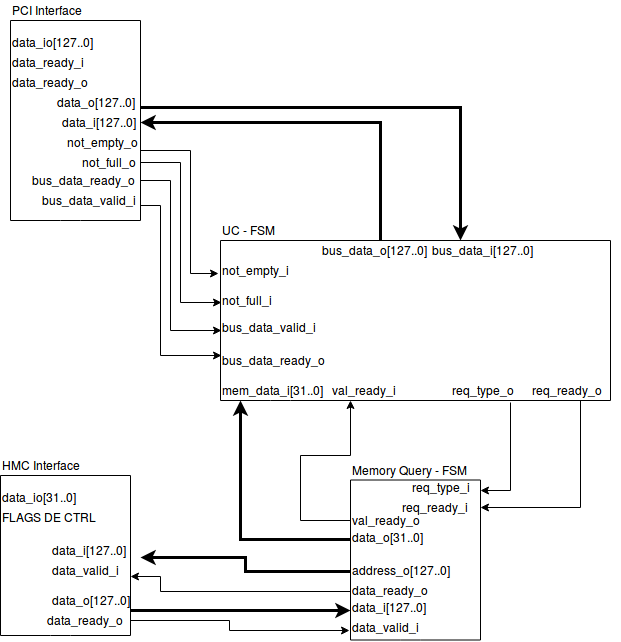
\includegraphics[scale = 0.5]{Figures/schema_bloc.png}
    \caption{Schema bloc of the project Top-Level}
    \label{fig:seqschema}
\end{figure}

\begin{description}
\item [PCI Interface] - This bloc is the interface between the \textsl{PCI Express Bus} and the FM-Index bloc. It receives short reads and command from a linked computed. In this interface, the FM-Index bloc is a slave, that wait for commands and data to start working. A FIFO is already implemented and this bloc consumes what is put into it. When a result is ready, it is placed in another FIFO that can be accessed by the computer master on the other end.
\item [HMC Interface] - Similarly to the previous bloc, this one is the interface between the board main memory and the FM-Index bloc. Only accessed through the \textsl{Memory Query} bloc, it is used to query data, may it be checkpoints entries, BWT entries of Sampled Suffix array elements. All transactions are 128bits wide and the interpretation of the received data in the \textsl{Memory Query} bloc.
\item [Memory Query] - This bloc is used by the FM-Index 
\end{description}


\section{VHDL Implementation}


\section{Test \& Validation}













